\documentclass[12pt,a4paper,openany]{report}
\usepackage[a4paper,margin=1in]{geometry}
\usepackage[T1]{fontenc}
\usepackage[utf8]{inputenc}
\usepackage{mathptmx}
\usepackage{setspace}
\usepackage{graphicx}
\usepackage{float}
\usepackage{booktabs}
\usepackage{array}
\usepackage{tabularx}
\usepackage{longtable}
\usepackage{xcolor}
\usepackage{hyperref}
\usepackage{caption}
\usepackage{tikz}
\usetikzlibrary{arrows.meta,positioning,shapes.geometric}
\usepackage{listings}
\usepackage{fancyhdr}
\usepackage{titlesec}
\usepackage{enumitem}
\usepackage{url}
\usepackage{placeins}

\hypersetup{colorlinks=true, linkcolor=black, urlcolor=blue, citecolor=black}
\onehalfspacing
\raggedbottom
\setlength{\parindent}{0pt}
\setlength{\parskip}{6pt}
\renewcommand{\arraystretch}{1.15}
\captionsetup{font=bf, labelfont=bf}
\urlstyle{same}

\definecolor{codegray}{RGB}{246,248,250}
\definecolor{codeborder}{RGB}{210,215,220}
\lstdefinestyle{reportcode}{
  backgroundcolor=\color{codegray},
  basicstyle=\ttfamily\small,
  breaklines=true,
  frame=single,
  framerule=0.4pt,
  rulecolor=\color{codeborder},
  columns=fullflexible,
  keepspaces=true,
  showstringspaces=false,
  tabsize=2
}
\lstset{style=reportcode}

\pagestyle{fancy}
\fancyhf{}
\fancyhead[L]{23AIML049}
\fancyhead[R]{Agentic Requirement Analyzer -- Internship Report}
\fancyfoot[L]{CSPIT, CHARUSAT}
\fancyfoot[C]{\thepage}
\fancyfoot[R]{Department of AIML}
\renewcommand{\headrulewidth}{0.4pt}
\renewcommand{\footrulewidth}{0.4pt}
\setlength{\headheight}{15pt}

\titleformat{\chapter}[display]
  {\normalfont\bfseries\centering\Large}
  {CHAPTER \thechapter}
  {0.5em}
  {\Large}
\titlespacing*{\chapter}{0pt}{-5pt}{14pt}
\titleformat{\section}{\normalfont\bfseries\large}{\thesection}{1em}{}
\titleformat{\subsection}{\normalfont\bfseries}{\thesubsection}{1em}{}

\newcommand{\reporttitle}{AGENTIC REQUIREMENT ANALYZER}
\newcommand{\subtitle}{Autonomous Multi-Agent AI System for Software Requirement Analysis and User Story Generation}
\newcommand{\student}{HARI PATEL}
\newcommand{\rollno}{23AIML049}
\newcommand{\internalguide}{Prof. Hardik Jaiswal}
\newcommand{\externalguide}{Mr. Pallav Mamtora}
\newcommand{\externaltitle}{CEO}
\newcommand{\company}{Techmicra IT Solutions}
\newcommand{\hod}{Dr. Nirav Bhatt}

\newcommand{\mFR}{20 / 16 / 28}
\newcommand{\mNFR}{6 / 11 / 9}
\newcommand{\mUS}{20 / 16 / 28}
\newcommand{\mAC}{20 / 17 / 28}
\newcommand{\mAMB}{5 / 5 / 3}
\newcommand{\mRISK}{7 / 10 / 10}
\newcommand{\mTIME}{68 / 83 / 118}
\newcommand{\mPY}{24}
\newcommand{\mJS}{8}

\begin{document}
\pagestyle{fancy}
\pagenumbering{roman}
\setcounter{page}{6}
\addtocontents{toc}{\protect\contentsline {chapter}{Company / Organization Certificate}{ii}{}}
\addtocontents{toc}{\protect\contentsline {chapter}{Declaration by the Candidate}{iii}{}}
\addtocontents{toc}{\protect\contentsline {chapter}{Acknowledgement}{iv}{}}
\addtocontents{toc}{\protect\contentsline {chapter}{Abstract}{v}{}}
\tableofcontents
\clearpage
\listoffigures
\clearpage

\pagestyle{fancy}
\pagenumbering{arabic}

% ==================== CHAPTER 1 ====================
\chapter{INTRODUCTION}

\section{Background of Internship}
This report documents a four-week summer internship carried out at
\textbf{\company}, a software development organization, under the
subject Summer Internship -- II (AIML402). The internship was structured
around a single, complete project rather than a rotation of small tasks,
which allowed the internship to go from initial design to a working,
end-to-end system within the four-week period.

\section{Company Overview}
\company\ is a software development organization that builds custom
software and AI-driven solutions for its clients. The internship was
supervised externally by \externalguide, \externaltitle\ of the company,
who guided the choice of project and reviewed progress through the
internship period.

\section{Problem Statement}
Before development begins, a business analyst typically has to read a
client's requirement document, identify the actors and features involved,
separate functional requirements from non-functional ones, translate them
into Agile user stories with acceptance criteria, and flag anything vague
or contradictory. This process is manual, slow, and inconsistent between
analysts. The goal of this internship project was to automate this
workflow using an agentic AI pipeline, where each step is handled by a
dedicated, specialized agent rather than a single large prompt.

\section{Objectives}
\begin{itemize}[leftmargin=*]
\item Design a multi-agent pipeline that mirrors how a business analyst
  would actually break down a requirement document.
\item Learn and apply LangGraph for deterministic, sequential agent
  orchestration.
\item Build a working FastAPI backend and React frontend around the
  pipeline.
\item Use vector similarity search (FAISS) to give the ambiguity-detection
  agent concrete grounding rather than asking an LLM to judge vagueness
  from nothing.
\item Produce a single, structured requirement analysis report as the
  final output of the pipeline.
\end{itemize}

\section{Scope}
The project was scoped to a four-week internship and focused entirely on
the requirement-analysis pipeline: document upload and parsing, requirement
extraction and classification, user story and acceptance criteria
generation, ambiguity detection, report assembly, and a frontend to
interact with the pipeline. Deployment infrastructure, multi-user
accounts and integrations with external issue trackers (e.g. Jira) were
intentionally left out of scope for this internship.

\section{Internship Timeline}
The four-week internship followed the same progressive order reflected in this
report: requirement understanding first, followed by architecture,
implementation, integration and testing.

\begin{table}[H]
\centering
\caption{Week-by-Week Internship Timeline}
\label{tab:timeline}
\begin{tabularx}{\textwidth}{|p{2.2cm}|X|}
\hline
\textbf{Week} & \textbf{Work Completed} \\
\hline
Week 1 & Studied the problem domain, finalized project objectives, prepared sample requirement documents and established the backend/frontend development environment. \\
\hline
Week 2 & Implemented document parsing, requirement extraction and functional/non-functional classification with structured JSON contracts. \\
\hline
Week 3 & Added user-story generation, Given/When/Then acceptance criteria, Sentence-Transformers embeddings and FAISS-based ambiguity detection. \\
\hline
Week 4 & Integrated FastAPI endpoints, React report rendering, SQLite run persistence, automated tests, execution verification and technical documentation. \\
\hline
\end{tabularx}
\end{table}

% ==================== CHAPTER 2 ====================
\chapter{REQUIREMENT ANALYSIS AND TECHNOLOGY STACK}

\section{Functional Requirements}
\begin{table}[H]
\centering
\caption{Functional Requirements of the System}
\label{tab:functional}
\begin{tabularx}{\textwidth}{|>{\raggedright\arraybackslash}p{3.6cm}|X|}
\hline
\textbf{Requirement Area} & \textbf{Description} \\
\hline
Document Upload & Accept a client requirement document in PDF, DOCX or TXT format through the web interface. \\
\hline
Document Parsing & Extract clean, structured text from the uploaded document regardless of source format. \\
\hline
Requirement Extraction & Identify actors, system features and constraints described in the document. \\
\hline
Requirement Classification & Separate extracted requirements into functional and non-functional categories. \\
\hline
User Story Generation & Convert functional requirements into Agile user stories with an assigned priority. \\
\hline
Acceptance Criteria Generation & Produce Given/When/Then acceptance criteria for every generated user story. \\
\hline
Risk and Ambiguity Detection & Flag vague or risky requirements and suggest a concrete rewording. \\
\hline
Report Assembly & Combine all agent outputs into one structured report with an executive summary. \\
\hline
Run History & Persist each analysis run so past reports can be revisited later. \\
\hline
\end{tabularx}
\end{table}

\section{Non-Functional Requirements}
\begin{table}[H]
\centering
\caption{Non-Functional Requirements of the System}
\label{tab:nonfunctional}
\begin{tabularx}{\textwidth}{|>{\raggedright\arraybackslash}p{3.6cm}|X|}
\hline
\textbf{Quality Attribute} & \textbf{Implementation Direction} \\
\hline
Reliability & Every agent degrades gracefully -- a failed LLM call or malformed JSON response falls back to an empty result and is logged, instead of crashing the pipeline. \\
\hline
Modularity & Each agent is a self-contained function with its own prompt, taking and returning a shared pipeline state, so agents can be built, tested and debugged independently. \\
\hline
Explainability & LangGraph's explicit state-machine model was chosen over a more autonomous framework (e.g. CrewAI) so that each agent hand-off is deterministic and traceable. \\
\hline
Usability & A React frontend shows pipeline progress and renders the final report in a readable, sectioned layout rather than raw JSON. \\
\hline
Persistence & Past analysis runs are stored in SQLite so a report is not lost after the browser session ends. \\
\hline
\end{tabularx}
\end{table}

\section{Technology Stack}
\begin{table}[H]
\centering
\caption{Technology Stack Summary}
\label{tab:techstack}
\begin{tabularx}{\textwidth}{|p{3.2cm}|X|}
\hline
\textbf{Area} & \textbf{Technologies} \\
\hline
Orchestration & LangGraph \texttt{StateGraph} (six nodes, linear edges) \\
\hline
Language Model & Groq API (llama-3.3-70b-versatile; openai/gpt-oss-120b for the final test runs) \\
\hline
Backend & Python 3.11, FastAPI \\
\hline
Frontend & React 18, Tailwind CSS \\
\hline
Document Parsing & pypdf (PDF), python-docx (DOCX) \\
\hline
Ambiguity Detection & Sentence-Transformers embeddings, FAISS similarity search \\
\hline
Persistence & SQLite \\
\hline
Version Control & Git and GitHub \\
\hline
\end{tabularx}
\end{table}
\FloatBarrier

% ==================== CHAPTER 3 ====================
\chapter{SYSTEM ARCHITECTURE}

\section{Pipeline Overview}
The system is built around a shared pipeline state that passes through six
agents in a fixed sequence. The pipeline is implemented as a compiled
LangGraph \texttt{StateGraph}~[2] in \texttt{backend/graph.py}: each agent is a node,
the nodes are joined by linear edges from \texttt{START} to \texttt{END}, and the
\texttt{errors} field uses an additive reducer so that warnings from every
agent are retained. Each agent reads the fields it needs and returns only
the fields it owns, which keeps intermediate output traceable.
Figure~\ref{fig:architecture} shows the complete pipeline.

\begin{figure}[H]
\centering
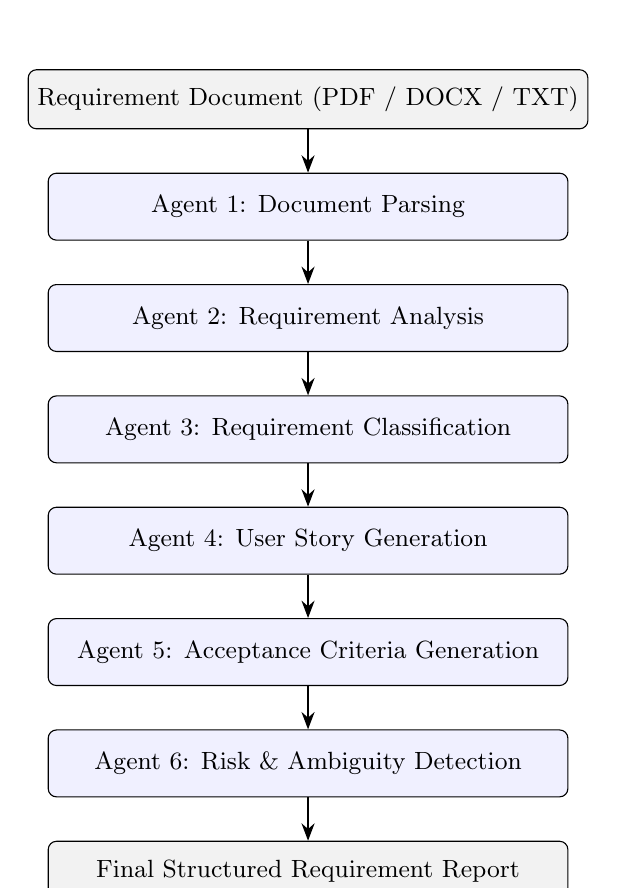
\begin{tikzpicture}[
  node distance=0.55cm and 0.9cm,
  every node/.style={font=\small},
  box/.style={draw, rounded corners=3pt, fill=blue!6, minimum width=6.6cm, minimum height=0.85cm, align=center},
  io/.style={draw, rounded corners=3pt, fill=gray!10, minimum width=6.6cm, minimum height=0.75cm, align=center},
  arr/.style={-{Stealth[length=2.2mm]}, thick}
]
\node[io] (doc) {Requirement Document (PDF / DOCX / TXT)};
\node[box, below=of doc] (a1) {Agent 1: Document Parsing};
\node[box, below=of a1] (a2) {Agent 2: Requirement Analysis};
\node[box, below=of a2] (a3) {Agent 3: Requirement Classification};
\node[box, below=of a3] (a4) {Agent 4: User Story Generation};
\node[box, below=of a4] (a5) {Agent 5: Acceptance Criteria Generation};
\node[box, below=of a5] (a6) {Agent 6: Risk \& Ambiguity Detection};
\node[io, below=of a6] (report) {Final Structured Requirement Report};
\draw[arr] (doc) -- (a1);
\draw[arr] (a1) -- (a2);
\draw[arr] (a2) -- (a3);
\draw[arr] (a3) -- (a4);
\draw[arr] (a4) -- (a5);
\draw[arr] (a5) -- (a6);
\draw[arr] (a6) -- (report);
\end{tikzpicture}
\caption{LangGraph pipeline architecture of the Agentic Requirement Analyzer.}
\label{fig:architecture}
\end{figure}

\section{Shared Pipeline State}
Every agent communicates through a single \texttt{PipelineState}
structure rather than passing ad-hoc arguments between functions. This
was one of the first design decisions made in the project, since it keeps
every agent independently testable.

\begin{lstlisting}
class PipelineState(TypedDict):
    raw_text: str
    filename: str
    actors: list[str]
    features: list[str]
    constraints: list[str]
    functional_requirements: list[str]
    non_functional_requirements: list[str]
    user_stories: list[dict]          # {feature, story, priority}
    acceptance_criteria: list[dict]   # {story_ref, given, when, then}
    risks: list[dict]                 # {requirement, reason, suggestion}
    ambiguities: list[dict]           # {requirement, reason, suggestion}
    errors: list[str]
\end{lstlisting}

\section{Agent Responsibilities}
\begin{longtable}{|p{3.3cm}|p{9.8cm}|}
\caption{Agent Responsibilities in the Pipeline}\\
\hline
\textbf{Agent} & \textbf{Responsibility} \\
\hline
Document Parsing & Detects the uploaded file type and extracts clean text, joining broken lines and stripping whitespace left over from PDF extraction. \\
\hline
Requirement Analysis and Classification & Reads the parsed text to identify actors, system features, and constraints, then classifies them into functional and non-functional requirements. \\
\hline
User Story Generation & Converts each functional requirement into an Agile user story with a priority level. \\
\hline
Acceptance Criteria Generation & Produces Given/When/Then acceptance criteria for every generated user story. \\
\hline
Risk \& Ambiguity Detection & Embeds each requirement, compares it against a seed corpus of known-vague phrases using FAISS, and asks the LLM to confirm the issue and suggest a concrete fix. \\
\hline
\end{longtable}

\FloatBarrier

% ==================== CHAPTER 4 ====================
\chapter{IMPLEMENTATION}

\section{Document Parsing Agent}
The parsing agent detects the file type from the upload's extension and
routes it to \texttt{pypdf} for PDF files or \texttt{python-docx} for DOCX
files, falling back to a direct read for plain text. Broken lines and
extra whitespace left over from PDF text extraction are cleaned before the
text is passed further down the pipeline.

\section{Requirement Analysis and Classification Agents}
Both agents prompt the Groq-hosted LLM to return \textbf{only valid JSON},
using a one-shot example inside the prompt to anchor the output format.
Each call is wrapped in a retry-once-then-fall-back pattern: if the model
returns malformed JSON, the agent retries a single time and, on repeated
failure, returns empty lists rather than raising an exception. This keeps
a single bad or unusual requirement document from crashing the whole
pipeline mid-run.

\section{User Story and Acceptance Criteria Agents}
For every functional requirement, the User Story agent generates an Agile
story in the ``As a / I want / So that'' format along with an inferred
priority. The Acceptance Criteria agent then takes each generated story
and produces Given/When/Then criteria, using the same retry/fallback
pattern as the earlier agents.

\section{Risk and Ambiguity Detection Agent}
This agent works differently from the others. A small seed corpus of
known-vague phrases (for example ``quickly'', ``user-friendly'', ``as
needed'') is embedded using a Sentence-Transformers model at module load
time [7] and indexed with FAISS [8]. For every requirement, the agent
embeds the requirement text and searches the index for the closest
known-vague phrases. If the similarity is above a threshold of 0.40, the
requirement and the matched phrase are passed to the LLM together, which
confirms the issue and proposes a concrete rewording -- for example,
replacing ``the system should respond quickly'' with a specific
response-time target. Separately, a rule-based detector classifies each
requirement into security, compliance, integration, performance or data
categories, with a severity and a mitigation, and populates the risks list.

\begin{lstlisting}
query_vector = normalize(embed(requirement))
scores, indexes = faiss_index.search(query_vector, k=3)
for score, index in zip(scores, indexes):
    if score >= similarity_threshold:
        matched_seed = seed_corpus[index]
        ambiguities.append(confirm_with_llm(requirement, matched_seed))
\end{lstlisting}

\section{Technical Code Review Findings}\label{sec:review}
A detailed review of the implementation and supplied screenshots
identified four engineering defects, all of which were fixed before
submission. First, the ambiguity detector used \texttt{faiss.IndexFlatIP}
without L2-normalized vectors, so scores were raw inner products; seed and
query embeddings are now normalized and scores are true cosine
similarities. Second, every top-$k$ match was forwarded to the LLM; matches
below the 0.40 threshold are now rejected. Third, the \texttt{risks} list
was never populated; risk detection is now separate from ambiguity
detection. Fourth, the acceptance prompt returned values that already
began with ``Given'', ``When'' and ``Then'', while the React renderer
prepended the labels again; the prompt now requests label-free values, the
backend strips any leading label, and the renderer adds each label once.

The upload endpoint was also hardened: only \texttt{.txt}, \texttt{.pdf}
and \texttt{.docx} files are accepted, files are stored under
server-generated names, uploads are limited to 5~MB, and \texttt{/analyze}
accepts only paths inside the upload directory.

\section{Report Assembly}
The final node in the graph combines the outputs of all six agents into
one structured report containing an executive summary, functional and
non-functional requirements, user stories, acceptance criteria, risks,
ambiguous requirements, and suggestions for improvement. Each completed
run is stored in SQLite so it can be revisited from the frontend's history
view.

\section{Frontend}
The React and Tailwind frontend provides a drag-and-drop upload form, a
pipeline step indicator, a history sidebar, and a results view with summary
counters, labelled Given/When/Then blocks, ambiguity and risk panels, and
report export. Figure~4.1 shows the upload interface.

\section{API Endpoints}
The backend exposes the following endpoints for the frontend and manual
testing:

\begin{table}[H]
\centering
\caption{Backend API Endpoints}
\label{tab:api}
\begin{tabularx}{\textwidth}{|p{3.2cm}|X|}
\hline
\textbf{Endpoint} & \textbf{Purpose} \\
\hline
\texttt{GET /health} & Basic health check used to confirm the backend is running. \\
\hline
\texttt{POST /upload} & Accepts a PDF, DOCX or TXT file (max 5~MB) into \texttt{uploads/}. \\
\hline
\texttt{POST /analyze/step1} & Runs parsing, analysis and classification only. \\
\hline
\texttt{POST /analyze} & Runs the full pipeline and saves the report in SQLite. \\
\hline
\texttt{GET /runs} & Returns the saved run history. \\
\hline
\texttt{GET /runs/\{run\_id\}} & Returns one stored analysis result by ID (404 if missing). \\
\hline
\end{tabularx}
\end{table}

\begin{figure}[H]
\centering
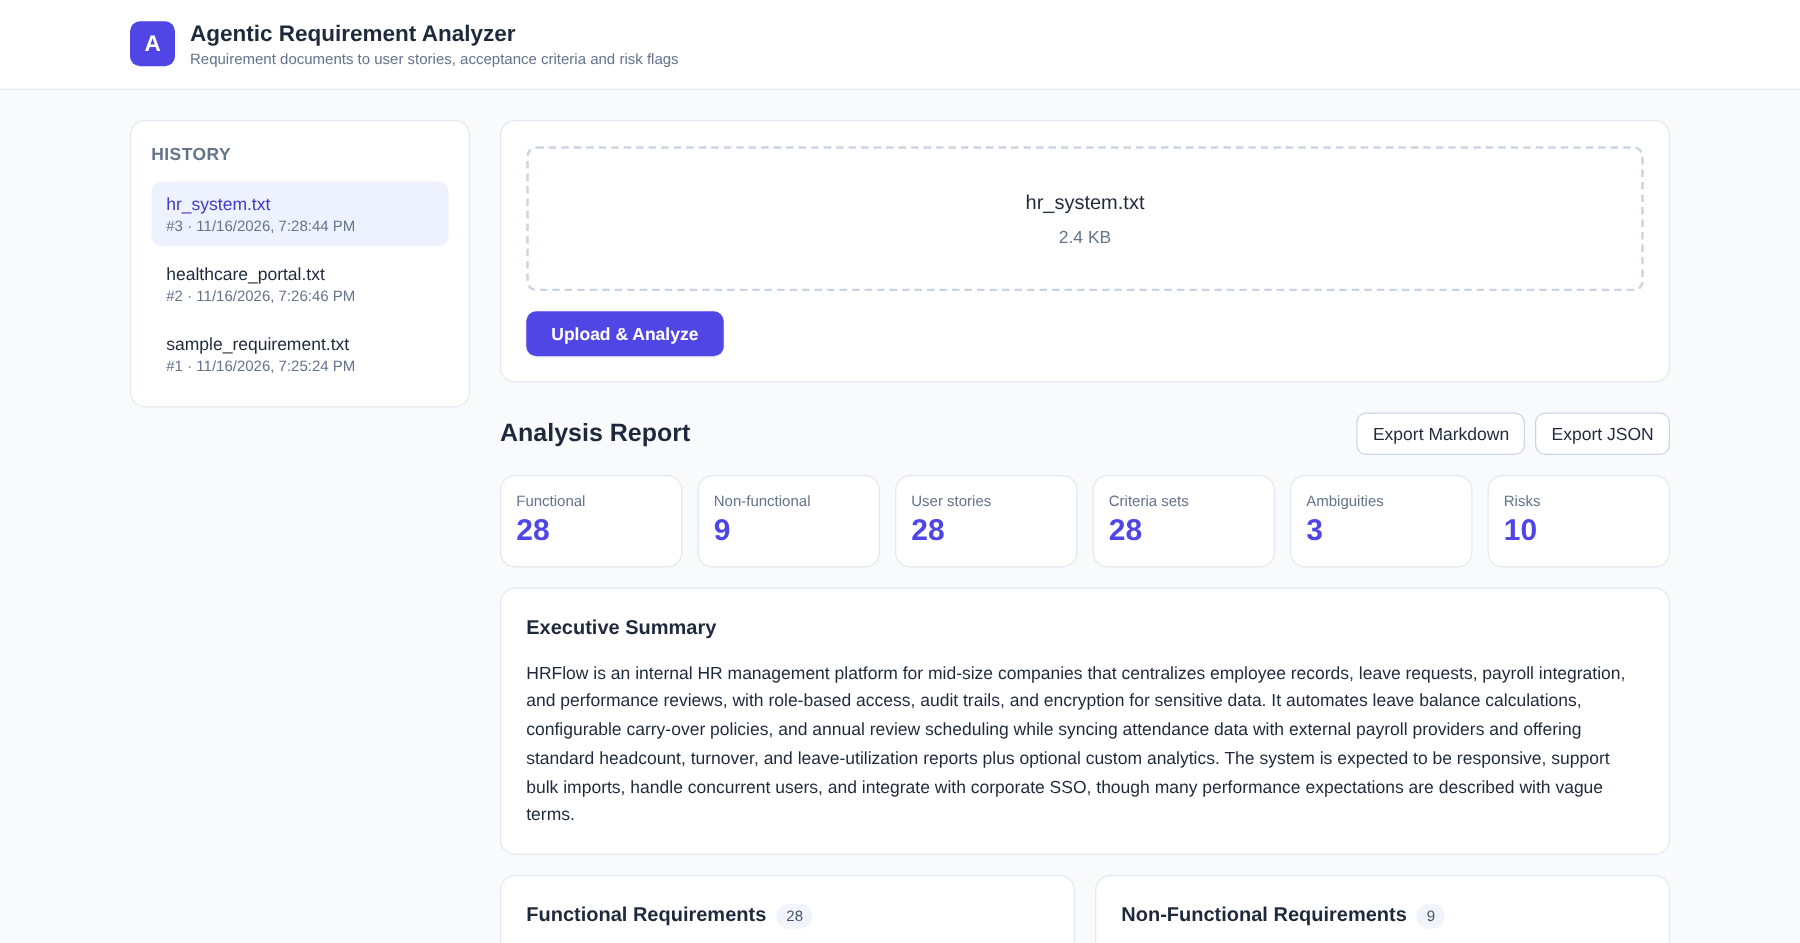
\includegraphics[width=429pt]{assets/upload_ui.png}
\caption{Document upload interface of the Agentic Requirement Analyzer frontend.}
\label{fig:uploadui}
\end{figure}

\FloatBarrier

% ==================== CHAPTER 5 ====================
\chapter{RESULTS AND TESTING}

\section{Testing Approach}
The completed pipeline was tested against sample requirement documents
from three different domains -- e-commerce, healthcare, and HR -- each
written with a deliberate mix of clear and vague requirements so that the
Risk \& Ambiguity agent had something meaningful to flag. Each document
was run through the full pipeline end to end via the \texttt{/analyze}
API endpoint, and the output of every agent was manually reviewed for
correctness before being considered complete.

\section{Sample Output}
Figure~\ref{fig:sampleoutput} shows the pipeline's JSON response for a
sample requirement document, and Figure~\ref{fig:reportview} shows the
same result rendered in the frontend's report view.

\begin{figure}[H]
\centering
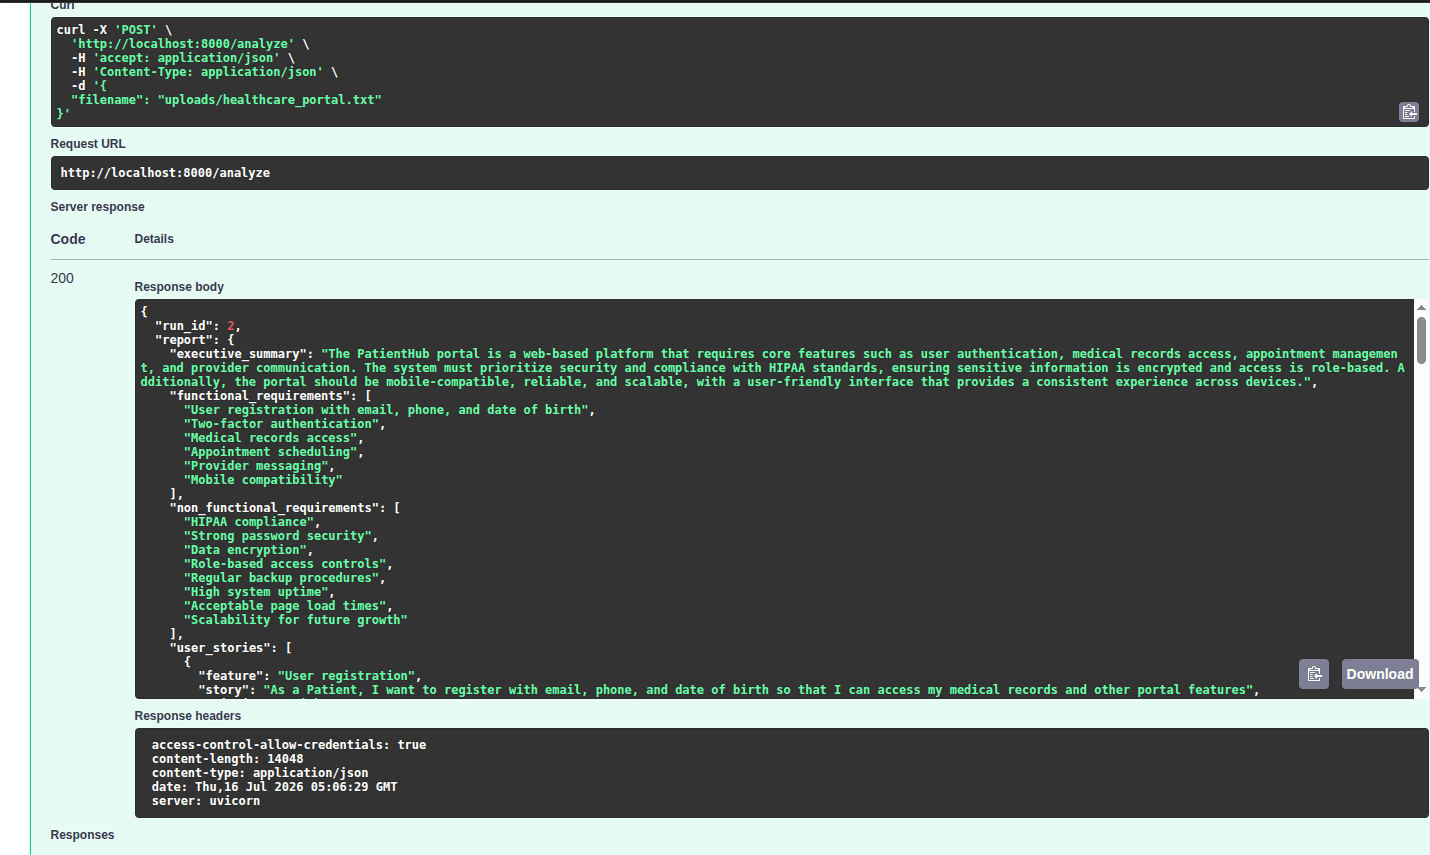
\includegraphics[width=0.9\textwidth]{assets/sample_json.png}
\caption{Sample \texttt{/analyze} API response for a test requirement document.}
\label{fig:sampleoutput}
\end{figure}

\begin{figure}[H]
\centering
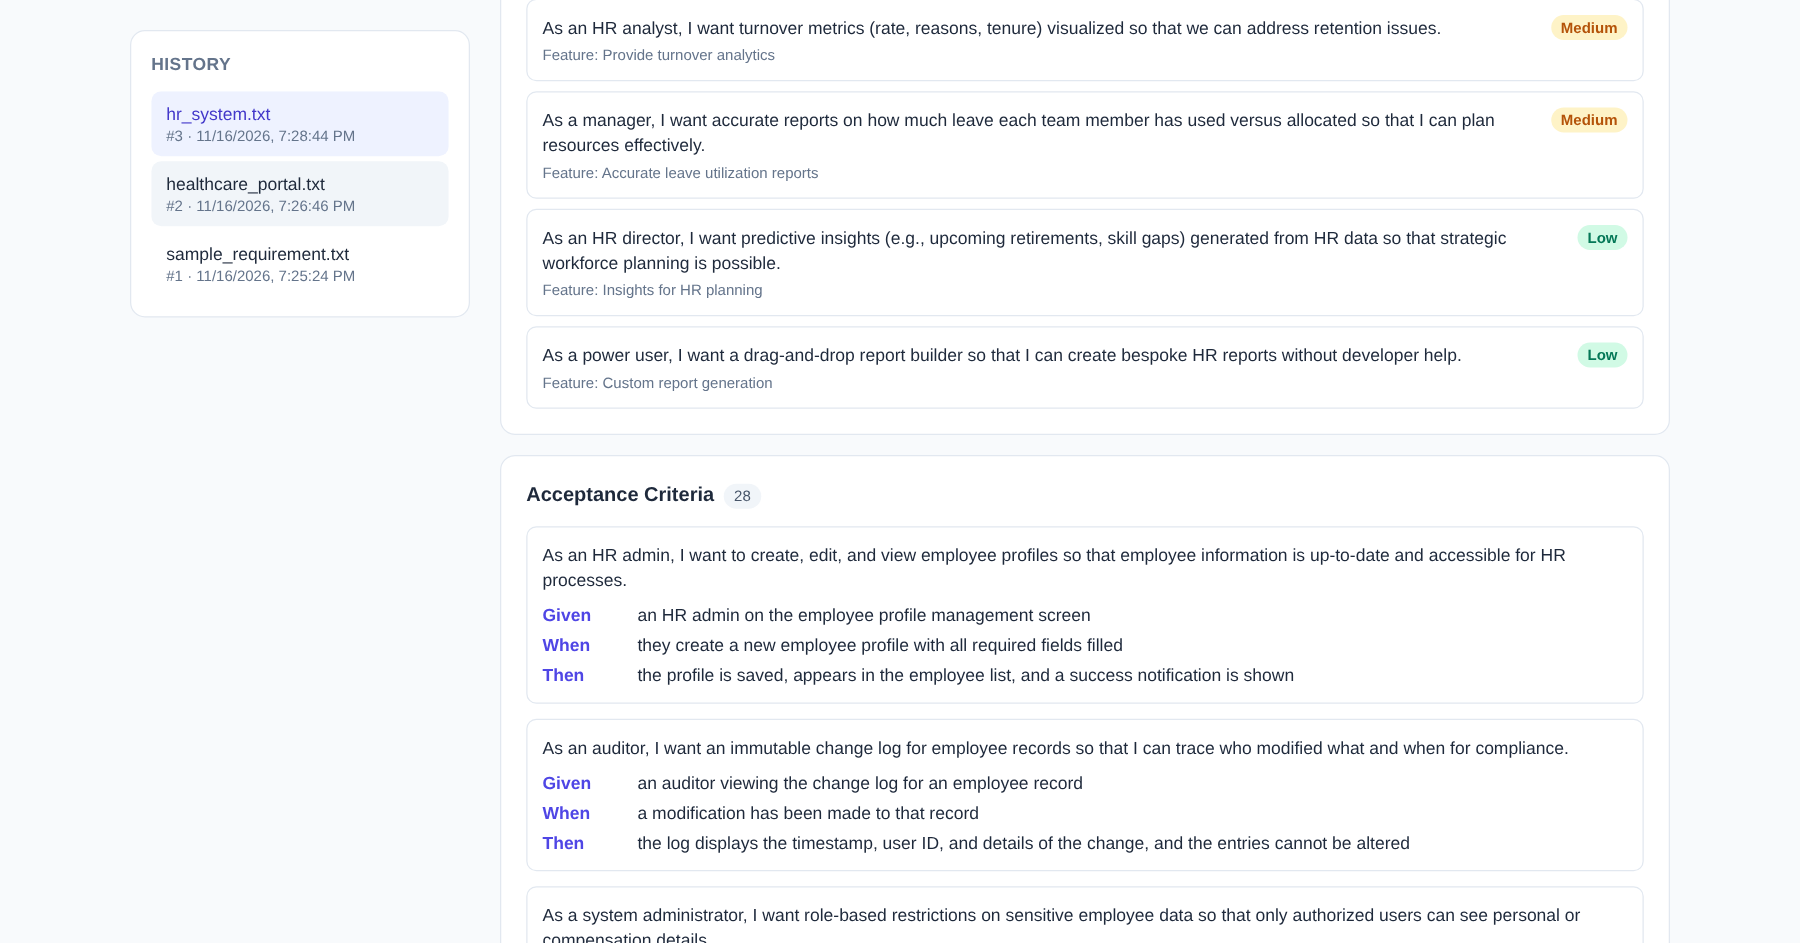
\includegraphics[width=0.9\textwidth]{assets/report_output.png}
\caption{Final structured report rendered in the frontend, showing requirements, user stories, acceptance criteria and flagged risks.}
\label{fig:reportview}
\end{figure}

\begin{table}[H]
\centering
\caption{Summary of Test-Run Results}
\label{tab:results}
\begin{tabularx}{\textwidth}{|p{5.6cm}|X|}
\hline
\textbf{Evaluation Metric} & \textbf{Observed Value (e-commerce / healthcare / HR)} \\
\hline
Functional requirements extracted & \mFR\ requirements \\
\hline
Non-functional requirements extracted & \mNFR\ requirements \\
\hline
User stories generated & \mUS\ stories \\
\hline
Acceptance criteria generated & \mAC\ criteria sets \\
\hline
Ambiguities flagged & \mAMB\ ambiguities \\
\hline
Risks flagged & \mRISK\ risks \\
\hline
End-to-end processing time & \mTIME\ seconds \\
\hline
\end{tabularx}
\end{table}

The values in Table 5.1 were measured from one controlled run of the final
pipeline on each of the three sample documents through the
\texttt{/analyze} endpoint, using \texttt{openai/gpt-oss-120b} on Groq
because \texttt{llama-3.3-70b-versatile} was no longer available.

\section{Technical Findings from Execution Evidence}
The FastAPI screenshots confirm successful HTTP 200 responses for full
analysis and run-history retrieval. The response structure contains a
run\_id and a nested report, which proves that report assembly and SQLite
persistence execute in the same workflow. The frontend confirms that the
backend/frontend contract is aligned, and the earlier formatting defect in
acceptance criteria was fixed (Section~\ref{sec:review}). The upload API now stores
files under server-generated names with an extension allow-list, a 5~MB
size limit and path confinement. The full pipeline is still synchronous, so
it should be moved to a background queue for concurrent use. The backend
is covered by \mPY\ \texttt{pytest} tests and the frontend by \mJS\
\texttt{vitest} tests, all passing.

\section{Observations}
Across the three sample documents, the Requirement Analysis and
Classification agents consistently separated functional from non-functional
requirements correctly. The Risk \& Ambiguity agent flagged the
intentionally vague phrasing in the samples (for example, unqualified
words like ``fast'' or ``secure'') and proposed specific, measurable
replacements; precision and recall were not measured, and the 0.40
threshold was chosen empirically on these three documents. The main source
of variation was in how granular the generated user stories were for very
broad requirements, which was addressed by refining the prompt to ask for
one story per distinct feature rather than per sentence.

\section{Project Repository}
The complete source code is available on GitHub, as shown in Figure 5.3.

\begin{figure}[H]
\centering
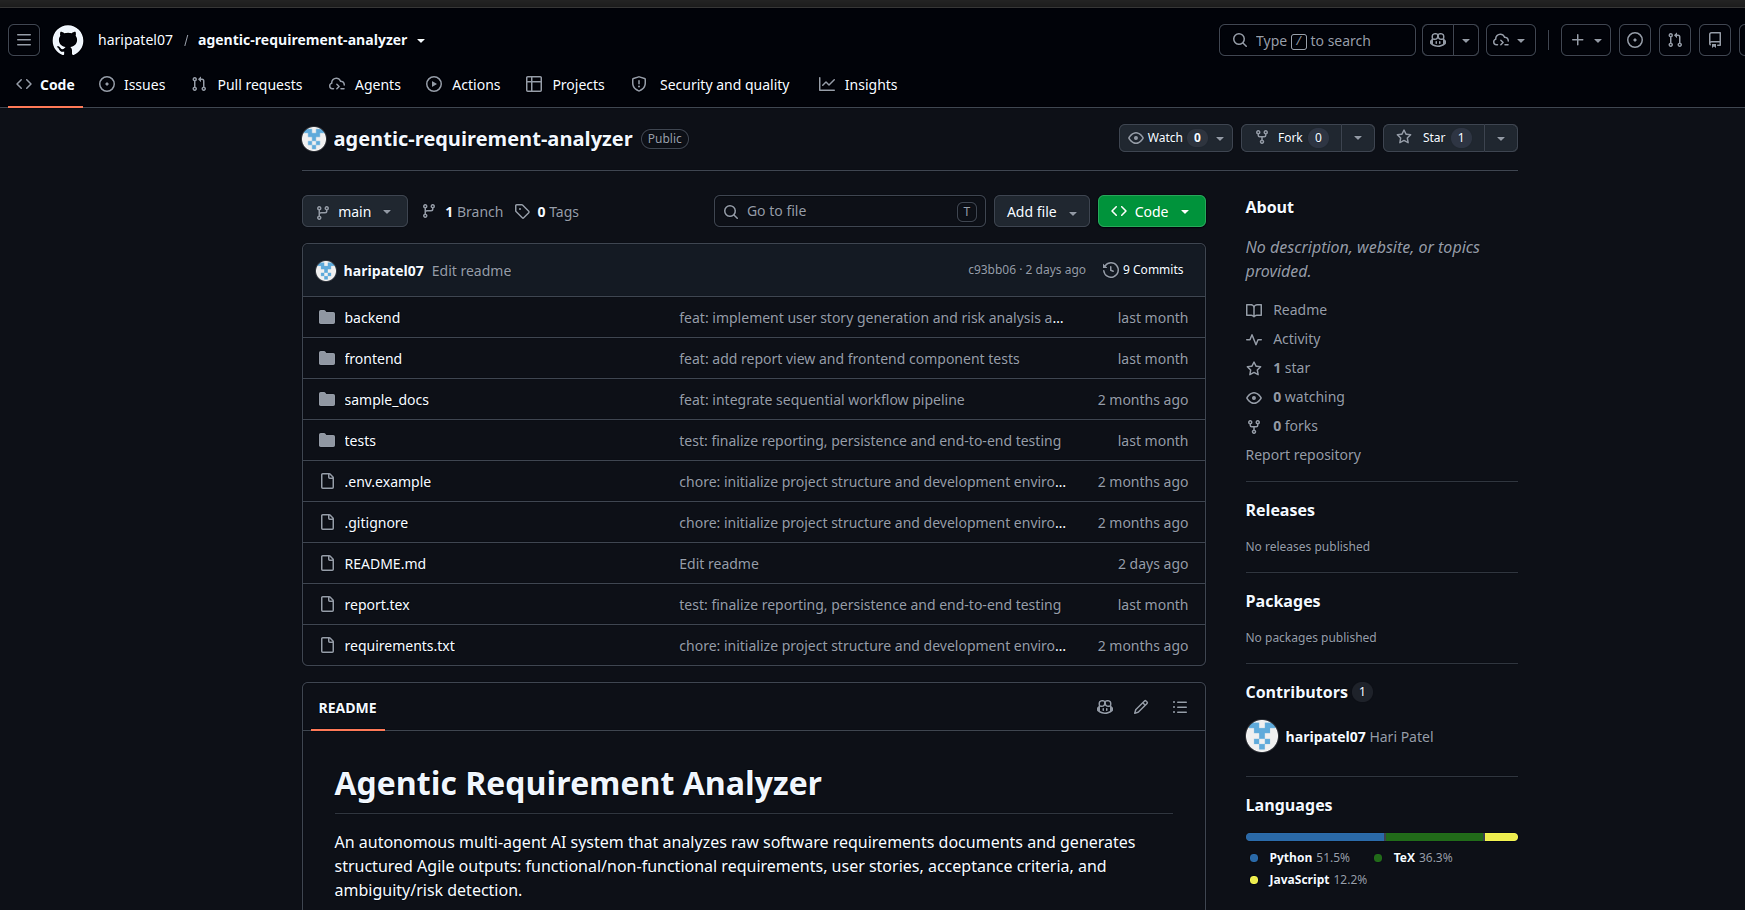
\includegraphics[width=0.9\textwidth]{assets/github_repo.png}
\caption{Agentic Requirement Analyzer repository on GitHub.}
\label{fig:githubrepo}
\end{figure}

\FloatBarrier

% ==================== CHAPTER 6 ====================
\chapter{CONCLUSION AND FUTURE SCOPE}

\section{Conclusion}
The objectives defined in Section 1.4 were achieved during the internship.
The modular six-stage analysis pipeline, implemented as a compiled
LangGraph \texttt{StateGraph}, together with multi-format document parsing,
actor/feature/constraint extraction, functional and non-functional
classification, user-story generation, acceptance-criteria generation,
FAISS-based ambiguity detection, rule-based risk detection, FastAPI
integration, React report rendering and SQLite persistence were fully
implemented, tested and demonstrated.

During implementation and review, I faced several technical challenges
that improved the quality of the project. I identified that the FAISS
\texttt{IndexFlatIP} vectors were not explicitly normalized, which meant
the scores could not safely be interpreted as cosine similarity, and that
the intended similarity threshold was described but not enforced before the
LLM confirmation step. In the frontend, acceptance-criteria fields already
contained the words ``Given'', ``When'' and ``Then'', while the renderer
added the same labels again. I fixed these issues, together with the
upload-endpoint weaknesses, and covered the fixes with automated tests.
The 0.40 similarity threshold was chosen empirically on three documents;
calibration on a labelled dataset remains future work.

Personally, the internship strengthened my ability to design agent
workflows, engineer prompts with strict JSON contracts, and implement
retry-once-then-fallback behaviour around unreliable model responses. I
gained practical experience with LangGraph orchestration, FastAPI endpoint
design, Sentence-Transformers embeddings, FAISS indexing, React integration
and persistent execution history. These skills connect directly with my
AIML coursework in natural language processing, machine learning
representations, software engineering and intelligent systems, while also
showing how model reasoning must be combined with validation, testing and
backend architecture to build a usable AI application.

\subsection{Limitations}
\begin{itemize}[leftmargin=*]
\item The current application has no authentication or authorization layer,
  so reports and uploaded documents are not protected by user identity or
  role-based access control.
\item The complete analysis pipeline runs synchronously inside the HTTP
  request, which limits concurrency and can cause long-running requests or
  timeouts.
\item SQLite persistence and the frontend are designed for a single-user
  demonstration and do not provide tenant separation, collaborative review
  or multi-user report ownership.
\item Risk detection is rule-based rather than model-based, and the
  ambiguity threshold has not been validated on a labelled dataset.
\end{itemize}

\section{Future Scope}
Beyond the scope of this internship, the system could be extended with Jira
or Azure DevOps integration to push generated user stories directly into a
sprint board, UML and database schema generation from the same parsed
requirements, multi-language requirement support, and an effort-estimation
agent that assigns story points based on similar past requirements.
Production hardening should additionally apply secure file-upload controls,
API-security practices and documented AI risk-management procedures in
accordance with OWASP and NIST guidance [17,18,19].

% ==================== REFERENCES ====================
\chapter*{REFERENCES}
\addcontentsline{toc}{chapter}{References}
\begin{enumerate}[leftmargin=*,label={[\arabic*]}]
\item Agentic Requirement Analyzer Code Repository,\\ \url{https://github.com/haripatel07/agentic-requirement-analyzer}
\item LangChain AI, LangGraph Documentation, \url{https://langchain-ai.github.io/langgraph/}
\item FastAPI Documentation, \url{https://fastapi.tiangolo.com/}
\item Groq API Documentation, \url{https://console.groq.com/docs}
\item pypdf Documentation, \url{https://pypdf.readthedocs.io/}
\item python-docx Documentation, \url{https://python-docx.readthedocs.io/}
\item Reimers, N., \& Gurevych, I., Sentence-BERT: Sentence Embeddings using Siamese BERT-Networks, EMNLP 2019.
\item Johnson, J., Douze, M., \& J\'egou, H., Billion-scale similarity search with GPUs, IEEE Transactions on Big Data, 2019.
\item Cohn, M., User Stories Applied: For Agile Software Development, Addison-Wesley, 2004.
\item Wiegers, K., \& Beatty, J., Software Requirements, Microsoft Press, 2013.
\item React Documentation, \url{https://react.dev/}
\item Tailwind CSS Documentation, \url{https://tailwindcss.com/docs}
\item SQLite Documentation, \url{https://www.sqlite.org/docs.html}
\item Pydantic Documentation, \url{https://docs.pydantic.dev/}
\item OpenAPI Specification, \url{https://spec.openapis.org/oas/latest.html}
\item Python Documentation, \url{https://docs.python.org/3/}
\item OWASP File Upload Cheat Sheet, \url{https://cheatsheetseries.owasp.org/cheatsheets/File_Upload_Cheat_Sheet.html}
\item OWASP API Security Top 10, \url{https://owasp.org/API-Security/}
\item NIST AI Risk Management Framework, \url{https://www.nist.gov/itl/ai-risk-management-framework}
\end{enumerate}

\end{document}